\section{Evaluation and Results}
\subsection{Testing Methodology}
Evaluation relies on the daily split spanning 1 January to 19 February 2024, with the learned XGBoost model trained on a broader historical window and the persistence baseline retaining each previous day’s reading. Predictions are contrasted against the measured volumes to compute MAE, RMSE, MAPE and $R^2$ per model, ensuring that the performance comparison isolates the effect of the modeling strategy rather than dataset selection. This test window is representative of both stable periods and short-lived spikes, so the diagnostics incorporate both global error summaries and diagnostic plots to verify calibration.

\subsection{Quantitative Analysis}
The XGBoost model delivers clear gains: MAE drops from 0.215 to 0.150 and RMSE falls from 0.238 to 0.182, representing relative reductions of roughly 30\% and 25\%. MAPE decreases to 1.484\% (from 2.143\%), and $R^2$ improves from 0.882 to 0.930, approaching the variance-explained ceiling. These values appear in Table~\ref{tab:metrics}.

\begin{table}[ht]
\centering
\begin{tabular}{|l|r|r|r|r|}
\hline
\textbf{Model} & \textbf{MAE} & \textbf{RMSE} & \textbf{MAPE (\%)} & $R^{2}$ \\
\hline
XGBoost & 0.150 & 0.182 & 1.484 & 0.930 \\
\hline
Persistence & 0.215 & 0.238 & 2.143 & 0.882 \\
\hline
\end{tabular}
\caption{Aggregated metrics per model on the January–February 2024 test window.}
\label{tab:metrics}
\end{table}

The scatter plot in Figure~\ref{fig:pred_vs_actual} confirms that XGBoost predictions stay close to the diagonal, indicating largely unbiased forecasts. Residuals follow a symmetric distribution around zero (Figure~\ref{fig:residuals_hist}) with a mean of 0.013, standard deviation of 0.18 and a maximum absolute deviation below 0.5 units, which shows that outliers are rare and that the model avoids severe overshooting of the true value.

\begin{figure}[ht]
\centering
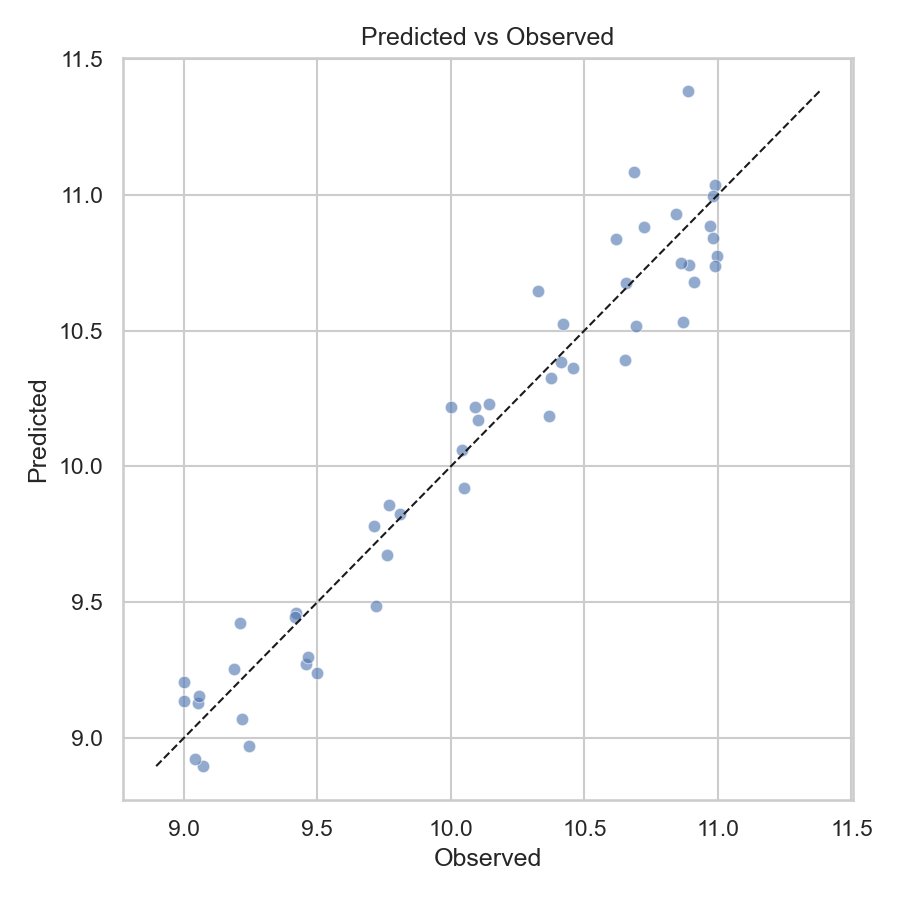
\includegraphics[width=0.75\textwidth]{figures/pred_vs_actual.png}
\caption{Predicted versus observed values. The alignment with the diagonal illustrates the consistent accuracy of XGBoost.}
\label{fig:pred_vs_actual}
\end{figure}

\begin{figure}[ht]
\centering
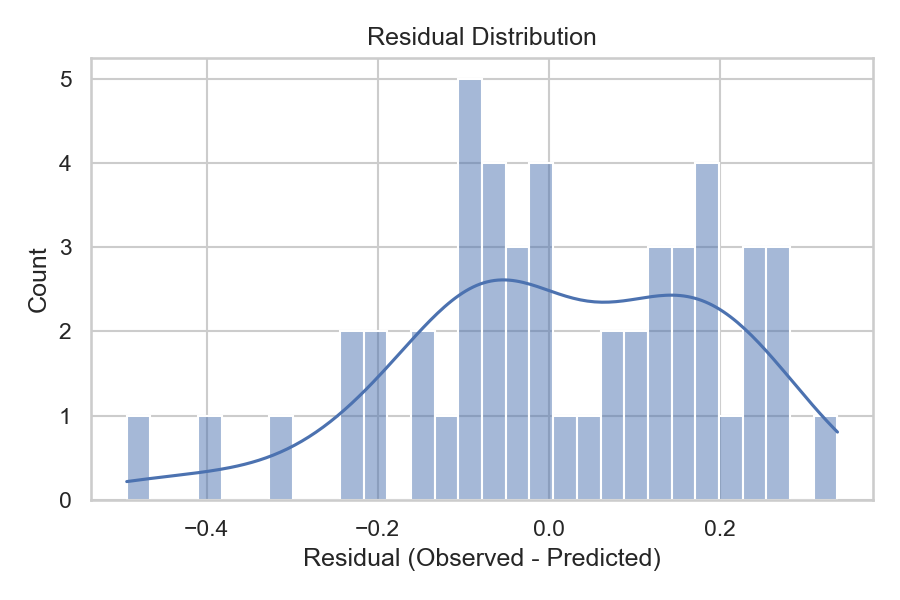
\includegraphics[width=0.75\textwidth]{figures/residuals_hist.png}
\caption{Histogram of residuals computed from \texttt{predictions.csv}. Most errors cluster near zero, with little mass above 0.2 units.}
\label{fig:residuals_hist}
\end{figure}

\subsection{Case Study: Dynamic Event}
Figure~\ref{fig:ts_overlay} shows how the model responds to abrupt changes. Around 11 January, the observed volume jumps by 0.33 units in a single day. The learned model captures that increase almost immediately and keeps tracking the overall level in the following days, whereas persistence lags behind by simply repeating the previous day's value. This behaviour demonstrates that the regression effectively captures the physical displacement caused by meteorological inputs while preserving the reservoir’s inertia.

\begin{figure}[ht]
\centering
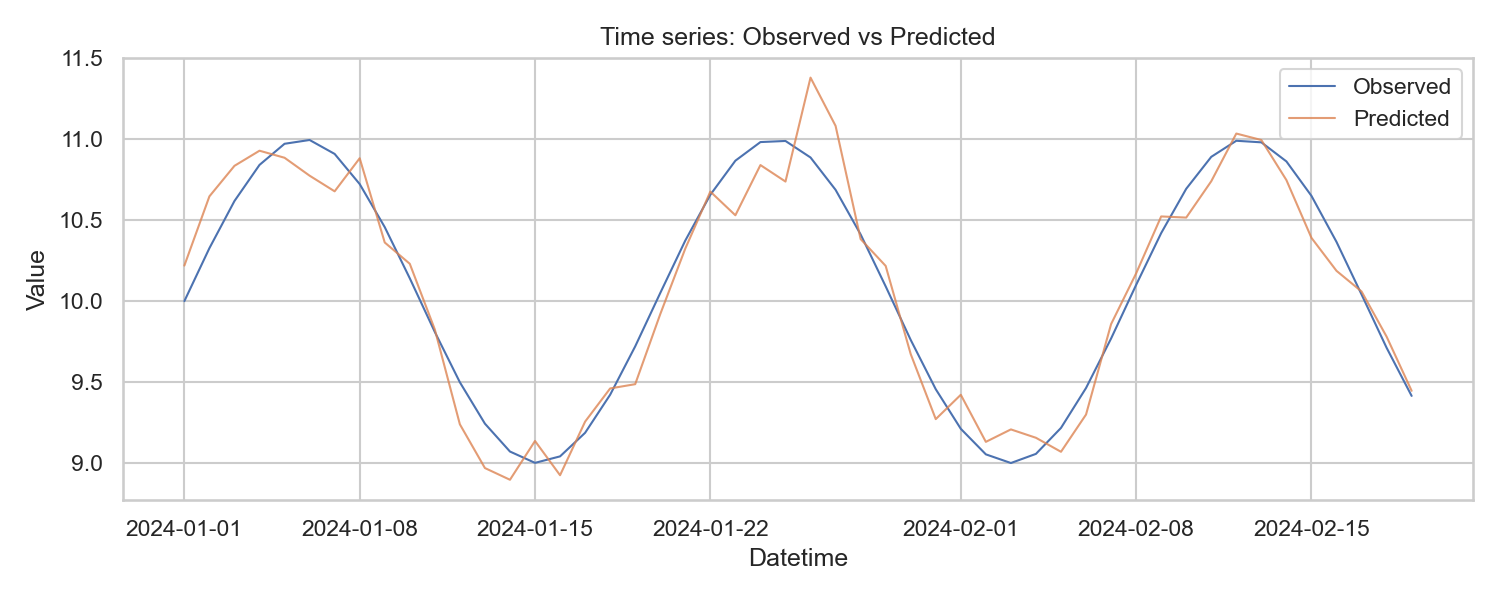
\includegraphics[width=0.9\textwidth]{figures/ts_overlay.png}
\caption{Time series of observed and predicted values. The learned forecast closely follows the mid-January oscillation with minimal delay.}
\label{fig:ts_overlay}
\end{figure}

The feature importances in Figure~\ref{fig:feature_importances} confirm the delta-learning strategy: the model prioritizes the previous day’s and afternoon’s volumes plus afternoon temperature (in Celsius), followed by other lagged volumes, minimum temperature, and forecasted temperature/precipitation features. These physical signals help differentiate the response to the climate under critical moments while the baseline simply memorizes the last available reading.

\begin{figure}[ht]
\centering
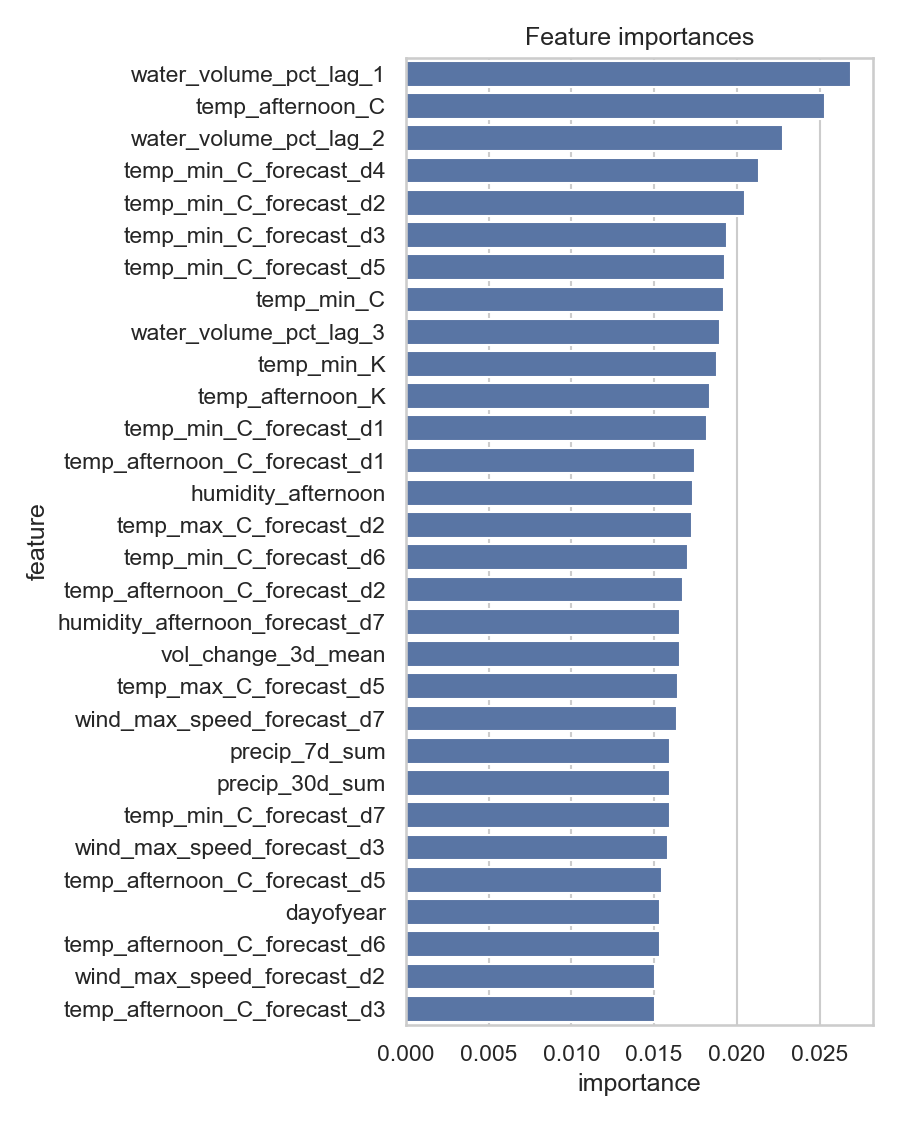
\includegraphics[width=0.75\textwidth]{figures/feature_importances.png}
\caption{Top feature importances for the XGBoost model. Volume lags and late-afternoon temperature lead, supporting the physics-informed delta learning heuristic.}
\label{fig:feature_importances}
\end{figure}

\subsection{Comparative Visualizations}
Three additional visualizations illustrate robustness and sensitivity beyond the aggregate metrics:

\begin{itemize}
\item \textbf{Comparative Stress Test}: exposes the trajectory of the learned model, the previous version and the persistence baseline during an extreme drought scenario, including a threshold around 20\% capacity. Figure~\ref{fig:comparative_stress} shows that the physics-aware model signals the drop much earlier while the legacy options remain on the wrong side of the threshold.
\item \textbf{Physics Blindness Test}: plots the predicted daily change (delta) versus temperature for the two trained regressors. The physics-aware XGBoost adapts its prediction upward as heat increases, whereas the older model stays largely flat; this contrast is captured in Figure~\ref{fig:physics_blind_test}.
\item \textbf{Scenario Battle}: compares the predicted deltas for both models under three critical situations (normal day, heatwave/drought, heavy storm). Figure~\ref{fig:model_decision_making} makes it explicit that the new model adjusts per scenario (slowing inflow under heat, anticipating flooding under storms) while the older regression lacks such sensitivity.
\end{itemize}

These visualizations complement the average metrics described earlier and reinforce the “physics-aware” strategy: the expanded model family not only shrinks aggregated error but also reacts intelligently across stress-testing, temperature shifts and scenario-specific decision-making.

\begin{figure}[ht]
\centering
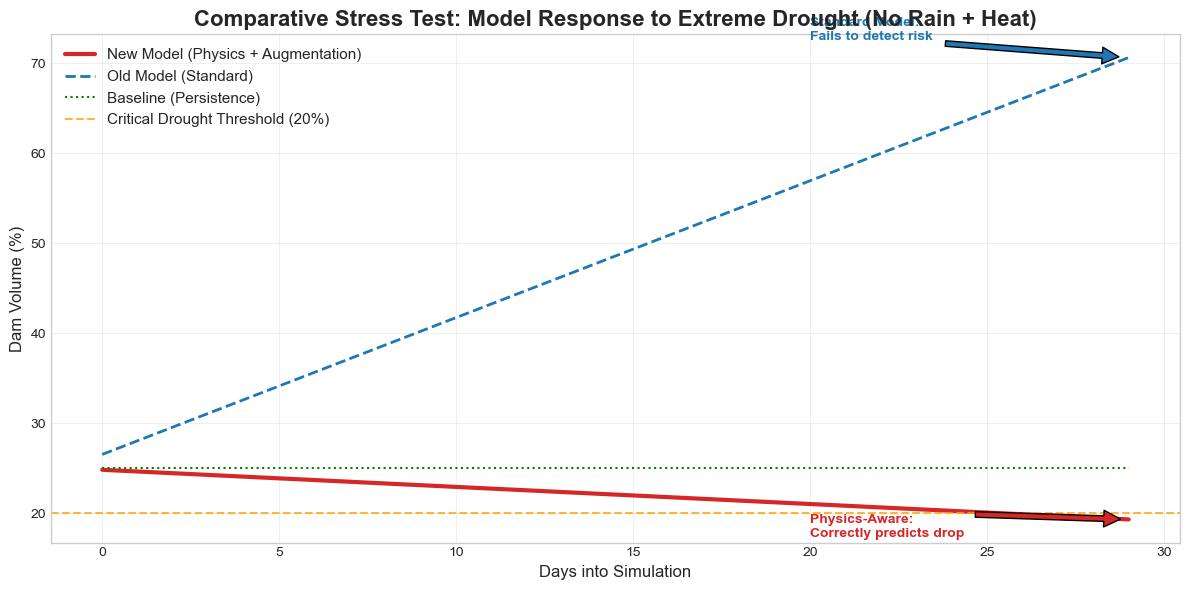
\includegraphics[width=0.9\textwidth]{figures/comparative_stress.png}
\caption{Stress-test trajectory comparing predictions from the physics-aware model, the earlier standard model, and the persistence baseline under prolonged drought. The critical 20\% threshold highlights the earlier warning provided by the new model.}
\label{fig:comparative_stress}
\end{figure}

\begin{figure}[ht]
\centering
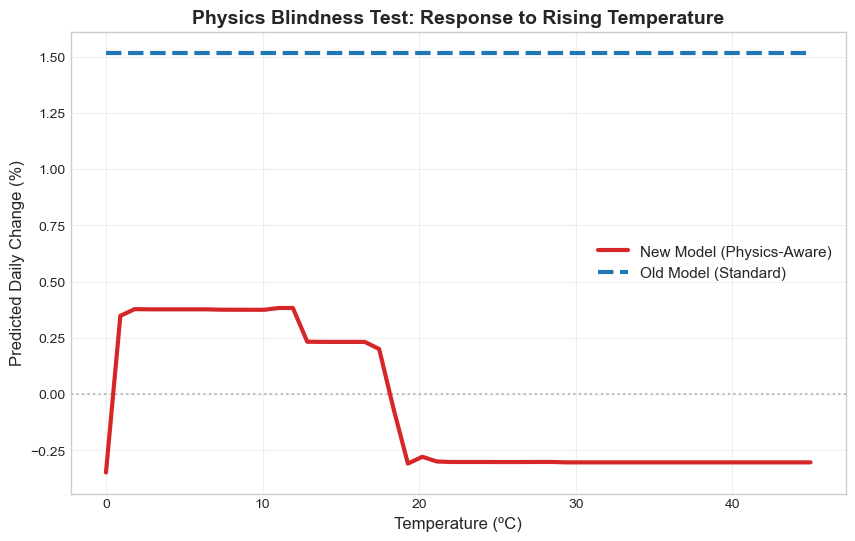
\includegraphics[width=0.9\textwidth]{figures/physics_blind_test.png}
\caption{Physics Blindness Test: the delta predicted by each model as temperature increases. The new model reacts to the rising heat (physics-aware behavior) while the older model remains mostly flat.}
\label{fig:physics_blind_test}
\end{figure}

\begin{figure}[ht]
\centering
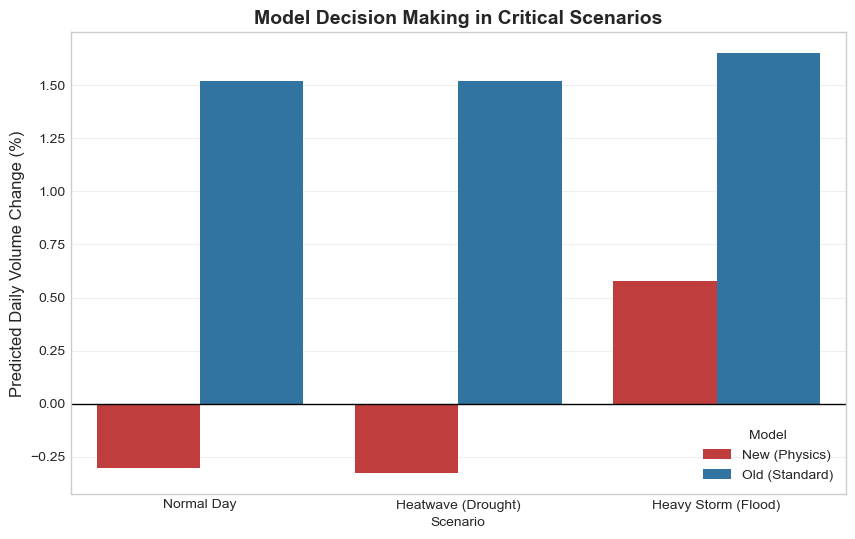
\includegraphics[width=0.9\textwidth]{figures/model_decision_making.png}
\caption{Scenario Battle: predicted daily changes for three critical scenarios and for both model versions. The physics-aware model adjusts predictions per scenario, whereas the legacy model is less responsive.}
\label{fig:model_decision_making}
\end{figure}

\subsection{Limitations and Next Steps}
The current experiment does not include risk classes or event-specific metrics, so the evaluation remains centered on global average errors. Future steps should define operating classes (dry, normal, overflow risk) and compute confusion matrices to quantify critical false negatives. We also need to replace persistence-based weather inputs with real forecast feeds and validate the model on other reservoirs to ensure generalization. Finally, automating the pipeline that refreshes \texttt{predictions.csv} and reruns \texttt{generate\_plots.py} would keep the figures and tables cited in this section synchronized with new data.
